\begin{comment}
\end{comment}

\chapter{Construction de codes correcteurs quantiques}

Dans le chapitre précédent, 
je me suis intéressé à la correction des erreurs lors de la communication classique.
Pour la suite de la thèse,
je vais quitter le régime classique pour m'intéresser au régime quantique.
Dans ce chapitre, 
je vais plus particulièrement m'intéresser à la protection de l'information 
dans un modèle quantique simplifié avant de présenter la conception d'une mémoire 
quantique au prochain chapitre.
Ce modèle simplifié, 
ressemblant au canal binaire symétrique présenté au premier chapitre, 
me permet de me concentrer sur la construction de codes correcteur d'erreurs quantique
sans avoir à me soucier des détails d'implémentation.

De façon similaire au scénario classique,
il est important de concevoir des codes correcteurs qui permettent 
de bien protéger l'information avec un nombre raisonnable de qubits supplémentaires.
En fait,
la présence des erreurs est l'un des facteurs limitant parmi les plus
important pour la réalisation de calculs quantiques.
Ainsi, 
la correction d'erreur ne se limite pas à des scénarios de communication 
comme dans la cas classique,
mais sera omniprésente dans un système de calcul quantique.

Cette importance accrue des erreurs dans les systèmes quantiques s'explique
principalement du fait qu'il s'agit de systèmes analogues plutôt que digital.
Un système est digital lorsqu'il chacun de ses éléments peut prendre un nombre fini
de valeurs. 
Dans le cas des ordinateurs classiques,
chaque bit prend soit la valeur 0 ou la valeur 1.
Ainsi,
il est possible d'utiliser une quantité continue comme une différence de potentielle 
pour représenter physiquement un bit tout en le protégeant des erreurs.
Par exemple,
le bit 0 peut être associé à un valeur de 0 volts et le bit 1 à une valeur de 5 volts.
Dans le cas où une valeur de 4.9 volts est mesurée, il y fortt probable que 
la valeur désirée est le bit 1.
Donc, en absence des perturbations externes présentent lors de la communicaton,
l'information classique est relativement robuste.

Au contraire, un système quantique est analogue puisqu'il existe une infinité d'états accessibles.
Par exemple, l'état d'un seul qubit est représenté par deux nombres complexes $a$ et $b$ 
avec la seule contraintre que $a^2 + b^2 = 1$. 
Une faible variation de ces paramètres représente un état différent et il est généralement
impossible de savoir si l'état du système est l'état désiré ou un état corompu.
De plus, l'accumulation de petites différences sur l'état de chacun des qubits peut complètement
changer le résultat d'un calcul.
Ce problème est si important que plusieurs scientifiques ont crus qu'il serait impossible




\section{Codes stabilisateurs et correction d'erreurs quantique}

\section{Problèmes de satisfaction de contraintes}

\section{Article : Une multitudes de codes stabilisateurs éparses}

Cet article ayant pour titre original \textit{Finite-rate quantum sparse codes aplenty}
a été soumis au journal Quantum a l'été 2022 et était toujours en
précessus de révision lors de la soumission de cette thèse.

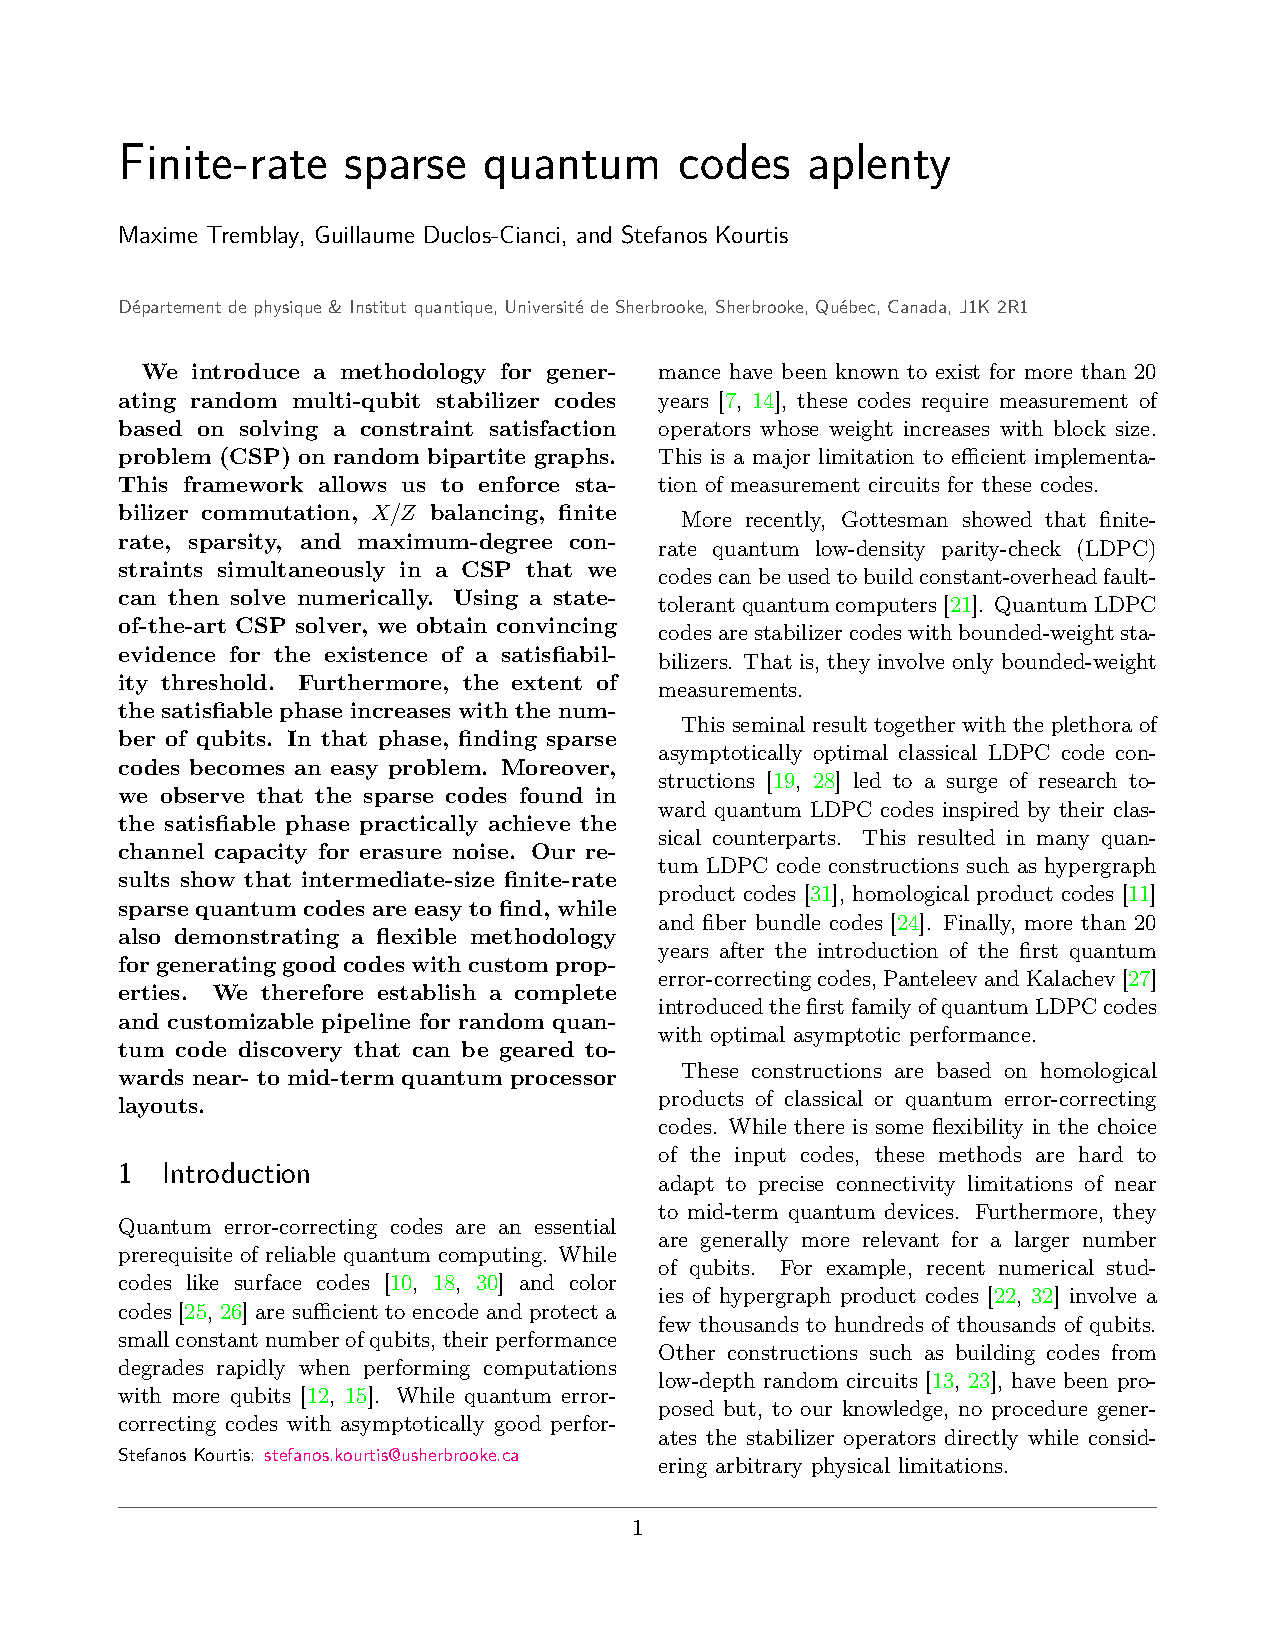
\includepdf[pages=-]{articles/sat_codes_construction.pdf}
